\usepackage[T1]{fontenc} % Codificación de las fuentes utilizadas
\usepackage[spanish]{babel} % Español como idioma principal del texto (permite hyphenation de palabras al final de una línea)


\usepackage{graphicx}
\usepackage{url}

\graphicspath{{Figures/}{Diagrams}{Chapters/}}  % Location of the graphics files (set up for graphics to be in PDF format)

\selectlanguage{spanish}

\setcounter{tocdepth}{1}

% Include any extra LaTeX packages required
\usepackage[square, numbers, comma, sort&compress]{natbib}  % Use the "Natbib" style for the references in the Bibliography
\usepackage{verbatim}  % Needed for the "comment" environment to make LaTeX comments
\usepackage{vector}  % Allows "\bvec{}" and "\buvec{}" for "blackboard" style bold vectors in maths
\hypersetup{urlcolor=blue, colorlinks=true}  % Colours hyperlinks in blue, but this can be distracting if there are many links.
\usepackage{hyperref}
% \usepackage[pdfauthor={Diego Martín Arroyo},
%             pdftitle={Diseño e implementación de un sistema de computación distribuida con
% Raspberry Pi, y estudio comparativo del mismo frente a otras soluciones},
%             pdfsubject={Memora del Trabajo de Fin de Grado},
%             pdfproducer={XeLaTeX with hyperref},
%             pdfcreator={XeLaTeX},
%             pdfkeywords={Computación Paralela, Sistema Distribuido, Raspberry}
%             ]{hyperref}
%% ----------------------------------------------------------------

%% --------------------------------------------------------------------------------------------------------------------------------
%http://tex.stackexchange.com/a/85218/76599
\usepackage{fancyvrb}
\usepackage[dvipsnames]{xcolor}

% redefine \VerbatimInput
\RecustomVerbatimCommand{\VerbatimInput}{VerbatimInput}% Inclusión de archivos de texto plano
{fontsize=\footnotesize,
 %
 frame=lines,  % top and bottom rule only
 framesep=2em, % separation between frame and text
 rulecolor=\color{Gray},
 %
 label=\fbox{\color{Black}data.txt},
 labelposition=topline,
 %
 commandchars=\|\(\), % escape character and argument delimiters for
                      % commands within the verbatim
 commentchar=*        % comment character
}

\usepackage{listings} % Requerido para la inserción de código
%Listings command

\usepackage{float}
\newcommand*\lstinputpath[1]{\lstset{inputpath=#1}}
\lstinputpath{Code/}

\newcounter{undefinedreferences}
\setcounter{undefinedreferences}{0}

\newcommand{\citationneeded}[1][None]{\stepcounter{undefinedreferences}\textsuperscript{\color{blue} [Citation needed: #1]}}

\newcommand{\checkreferences}{
\ifnum\value{undefinedreferences} > 0
\begin{center}
\immediate\write18{wget -O Figures/protester.png -nc http://imgs.xkcd.com/comics/wikipedian_protester.png}
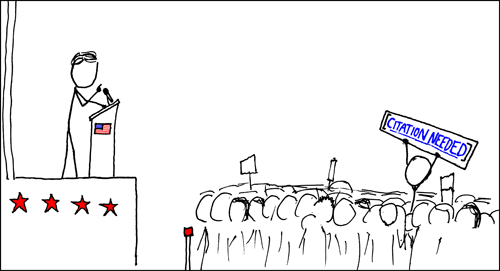
\includegraphics[width=\textwidth]{protester.png}\\
There are \arabic{undefinedreferences} undefined references
\end{center}
\else
No undefined references. Good!
\fi
}


%https://github.com/pads-fhs/LaTeX-Template-Thesis/blob/master/lststyles.tex
\lstdefinelanguage{JavaScript}{
  keywords={typeof, new, true, false, catch,%
    function, return, null, catch, switch, var,%
    if, in, while, do, else, case, break},
  ndkeywords={class, export, boolean, throw, implements, import, this},
  sensitive=false,
  comment=[l]{//},
  morecomment=[s]{/*}{*/},
  morestring=[b]',
  morestring=[b]"
}
\newcommand{\lstsetjavascript}{
  \lstset{
		language=JavaScript,
		breaklines=true,
		commentstyle=\textit,
		basicstyle=\ttfamily,
		keywordstyle=\bfseries,
		stringstyle=\ttfamily,
		showstringspaces=false,
		frame=single,
		tabsize=2
  }
}

\lstdefinelanguage{log}{
  keywords={typeof, new, true, false, catch,%
    function, return, null, catch, switch, var,%
    if, in, while, do, else, case, break},
  ndkeywords={class, export, boolean, throw, implements, import, this},
  sensitive=false,
  comment=[l]{//},
  morecomment=[s]{/*}{*/},
  morestring=[b]',
  morestring=[b]"
}
\newcommand{\lstsetlog}{
  \lstset{
		language=log,
		breaklines=true,
		commentstyle=\textit,
		basicstyle=\ttfamily,
		keywordstyle=\bfseries,
		stringstyle=\ttfamily,
		showstringspaces=false,
		frame=single,
		tabsize=2
  }
}

\lstloadlanguages{Java,XML, JavaScript, log}

\newcommand{\javascriptcode}[4]{
	\lstinputlisting[caption=#2,label=#1, firstline=#3, lastline=#4]{#1.json}
}

\newcommand{\logcode}[4]{
	\lstinputlisting[caption=#2,label=#1, firstline=#3, lastline=#4]{#1.log}
}

\usepackage[bottom]{footmisc} %The footnotes go at the bottom of t\usepackage{dtklogos}he page, instead next to the last line.
%Ajustes para Java
% \lstset{
% 	language=java,
%  	frame=single, % Un marco simple alrededor del código
%     basicstyle=\small\ttfamily, % Utilizar fuente true type pequeña
%     keywordstyle=[1]\color{Blue}\bf, % Funciones en negrita y azul
%     keywordstyle=[2]\color{Purple}, % Argumentos en morado
%     keywordstyle=[3]\color{Blue}\underbar, % Funciones personalizadas subrayadas en azul
%     identifierstyle=, % Nada especial acerca de identificadores
%     commentstyle=\usefont{T1}{pcr}{m}{sl}\color{Green}\small, % Los comentarios se renderizan en fuente pequeña verde
%     stringstyle=\color{Purple}, % Cadenas en morado
%     showstringspaces=false, % No se muestran los espacios entre cadenas
%     tabsize=5, % 5 espacios por tabulado
%     %
%     % Put standard Perl functions not included in the default language here
%     %morekeywords={rand},
%     %
%     % Put Perl function parameters here
%     %morekeywords=[2]{on, off, interp},
%     %
%     % Put user defined functions here
%     %morekeywords=[3]{test},\usepackage{dtklogos}
%    	%
%     morecomment=[l][\color{Blue}]{...}, % Line continuation (...) like blue comment
%     numbers=left, % Número de línea a la izquierda
%     firstnumber=1, % Número de línea comienza en 1
%     numberstyle=\tiny\color{Blue}, % Los números de línea son azules y pequeños
%     stepnumber=5, % Los números de línea van de 5 en 5
%     breaklines=true % Salto de línea si el texto no entra. See http://stackoverflow.com/a/1875803
% }

%\usepackage{xltxtra} % XeLaTeX logo. Yep, just that
%http://tex.stackexchange.com/a/73179/76599
\usepackage{metalogo}
%\usepackage{dtklogos} %BibTeX logo
\def\BibTeX{{\rm B\kern-.05em{\sc i\kern-.025em b}\kern-.08em
    T\kern-.1667em\lower.7ex\hbox{E}\kern-.125emX}}

\newenvironment{alignedDescription}[2][0pt]
  {\begin{list}{}%
    {\renewcommand\makelabel[1]{\textsf{\textbf{##1}}\hfil}%
     \settowidth\labelwidth{\makelabel{#2}}%
     \setlength\leftmargin{\labelwidth+\labelsep + #1}}}%
  {\end{list}}

\newenvironment{elements}
{\begin{quote}\itshape\centering\small}
{\end{quote}}

\newenvironment{cabstract}
{\begin{quote}\itshape\centering\small}
{\end{quote}}

%\usepackage[xindy]{glossaries}
%\newcommand{\chapterabstract}{1}{
%	\begin{center}
%	\small\textit
%	#1
%	\end{center}
%}

\usepackage{xcolor,colortbl}
\usepackage{float}
\graphicspath{{Figures/}}
\newcommand{\hmwkTitle}{Evaluación de herramientas} % Assignment title
\newcommand{\hmwkDueDate}{Jueves,\ 21\ de\ mayo\ de\ 2015}
\newcommand{\hmwkClassInstructor}{Rodrigo Santamaría} % Teacher/lecturer
\newcommand{\hmwkAuthorName}{Diego Martín Arroyo} % Your name
\newcommand{\hmwkSubject}{5} % Evaluation subject number

%----------------------------------------------------------------------------------------
%   TITLE PAGE
%----------------------------------------------------------------------------------------
\newcommand{\ordinalindicator}{\hspace{-1.5mm}$\phantom{a}^{\circ}$}
\title{\hmwkTitle\\Sujetos de evaluación n\ordinalindicator \hmwkSubject}
\author{\textbf{\hmwkAuthorName}}
\date{21 de mayo de 2015} % Insert date here if you want it to appear below your name

\begin{document}
\maketitle

\tableofcontents
\section{Descripción}

\begin{itemize}
	\item \textbf{Perfil}: Estudiante de la asignatura \textbf{Arquitectura de Computadores e Interacción Persona-Ordenador}.
	\item No conocían las herramientas previamente.
	\item Cuentan con experiencia en el desarrollo de aplicaciones con MPI en el marco de la Asignatura, así como nociones básicas de diseño de interacción.
\end{itemize}


\section{Introducción}

En la presente evaluación se ha realizado un recorrido de interacción a través de los aspectos fundamentales del sistema, evaluando la opinión del sujeto como potencial usuario del sistema y su criterio respecto al diseño de interfaces gráficas de usuario.

\section{Evaluación}

\subsection{Status monitor}
La evaluación comienza con el análisis de la herramienta \textbf{Status monitor}. Se realizan críticas a la disposición de los elementos de la interfaz, en particular textos que escapan su contenedor. Recomienda añadir una leyenda sobre los colores en los gráficos de memoria y \textit{swap}. Respecto a la información presentada, considera que es suficiente, sugiriendo únicamente añadir una monitorización del tráfico de red, el tiempo durante el que el sistema ha estado conectado (\textit{uptime}) y gráficos que muestren un histórico de los valores observados. En la salida del comando \textbf{top} sugiere indicar el porcentaje de CPU que consume cada proceso.

Respecto a la solución propuesta para aceptar los certificados autofirmados o con un campo \textbf{CN} inválido, considera que es la mejor solución posible.

\subsection{Deployer}

El sujeto considera que la interfaz permite realizar de forma sencilla las tareas para las que ha sido diseñada, si bien eliminaría una serie de componentes:

\begin{itemize}
	\item Considera que la barra de progreso que representa la subida no debería mostrarse hasta que no comience la misma. Cree que puede crear confusión entre los usuarios.
	\begin{figure}[H]
	\centering
	
\includegraphics[width=0.4\textwidth]{progressbar}
	\caption{Estado de la barra de progreso antes de realizar la subida}
	\label{progressbar}
	\end{figure}

	\item Respecto a la fase de despliegue, cree que una mejora sustancial sería la adición de un mensaje de estado en cada nodo con el estado de la misma. También considera importante eliminar los paneles para la realización de la subida una vez que esta haya sido llevada a cabo (actualmente los elementos se mantienen para posibilitar realizar más despliegues con los mismos elementos).
\end{itemize}
\subsection{Logger}

Valora la herramienta positivamente, sugiriendo únicamente la adición de un botón de interrupción de la ejecución.

\subsection{General}

Sugiere la adición de un icono representativo del sistema, así como modificar el esquema de colores de algunos elementos y cambiar el tamaño de varios elementos, a fin de hacerlos más significativos.


\section{Conclusiones}

A raíz de esta sesión se extraen las siguientes conclusiones y los caminos de actuación:

\begin{itemize}
	\item Se aceptan todas las sugerencias estéticas.
	\item Implementar gráficas para reflejar el histórico.
	\item Detención de procesos desde la máquina remota en el \textbf{logger}.
	\item Añadir información sobre el \textit{uptime}.
	\item Adición de los datos propuestos al \textbf{Status Monitor}.
	\item Mantener el mecanismo de validación de certificados dado.
\end{itemize}


\end{document}
